\documentclass[../main.tex]{subfiles}
\begin{document}

\section{Verfahren}

\subsection{Datenerfassung}
Ziel ist ein digitales Abbild von einem realen Objekt zu erstellen.
Als Grundlage für dieses Abbild arbeite ich in diesem Fall mit Pointclouds 
die mithilfe eines Laserscanners aufgenommen wurden. Auch andere Möglichkeiten
Pointclouds zu erhalten sind denkdar und sollten mit dem Verfahren 
kompatibel sein.

\subsection{Scanner}
Der von mir eingesetze Scanner kann in einer Linie mit einer maximalen Länge 
die abstände zu einem Objekt messen.
Um das ganze Objekt zu erfassen muss der Scanner also linear über das Objekt 
bewegt werden. 
Hierfür wurde eine CNC-Fräse benutzt, beziehungsweise die 
verschiebungseigenschaften von einer.
Hier ist es wichtig die Vorlaufgeschwindigkeit der Fräse in Abhängigkeit von der
Frequenz des Scanners zu wählen. 
Ist die Geschwindigkeit zu gering nimmt der Scanner mehrere Aufnahmen von der
selben Linie auf, ist sie zu hoch werden Koordinaten auf dem Objekt übersprungen
und die Auflösung der resultieren Pointcloud sinkt.
\begin{figure}[h]
    \centering
    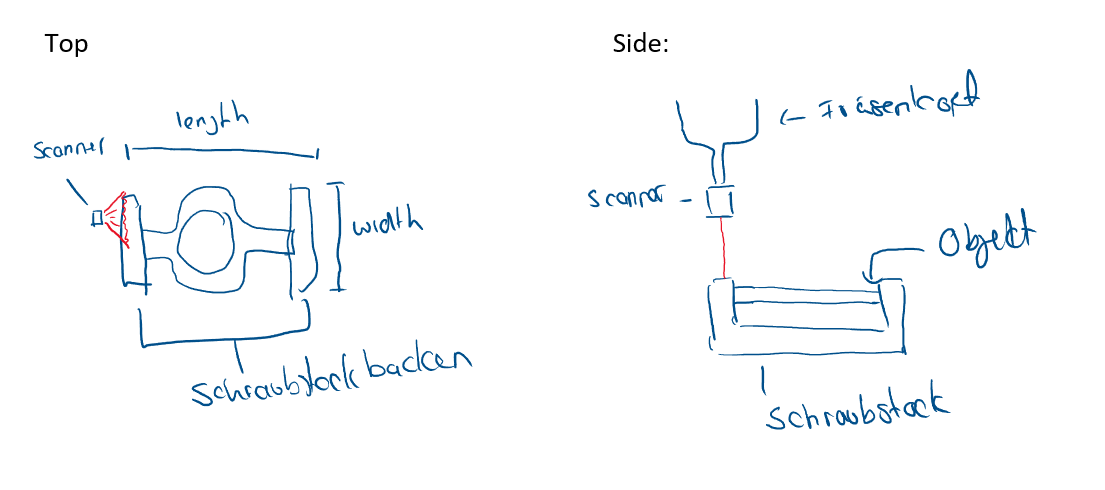
\includegraphics[height=200pt]{images/versuchsaufbau_sketch.PNG}
    \caption{Versuchsaufbau}
    \label{fig:versuchsaufbau}
\end{figure}


TODO: Berechnung für die Geschwindigkeit einfügen

In \ref*{fig:versuchsaufbau} ist der Versuchsaufbau skizziert.
Der Fräsenkopf wird in Richtung der Länge und Breite des Objekts verschoben.
Die gesamte Länge des Objekts kann also erfasst werden in dem Scanner 
beziehungsweise Fräsenkopf in X-Richtung bewegt wird. In dieser Bewegung 
ist die Limiterung einmal die maximale Länge des Fräsenachse, und außerdem der
verfügbare Speicher auf dem Computer der die Pointcloud aufnimmt.
In Y-Richtung sind wir durch die maximale Scannerbreite begrenzt. Diese ist, 
je nach Scanner, relativ klein.
Um auch Objekte Scannen zu können die breiter sind als die Scannerbreite werden
mehrere Scans erstellt, zwischen denen der Scanner immer in Y-Richtung 
verschoben wird. Die Länge der Verschiebung sollte kleiner als die 
Scannerbreite sein, damit eine überlappung entsteht die genutzt werden kann 
um die Pointclouds wieder zusammenzufügen. So können Pointclouds aufgenommen 
werden die dann im 2. Schritt wieder zu einem digitalen Abbild zusammengefügt 
werden.

\begin{wrapfigure}{l}{0.4\textwidth}
    \begin{center}
        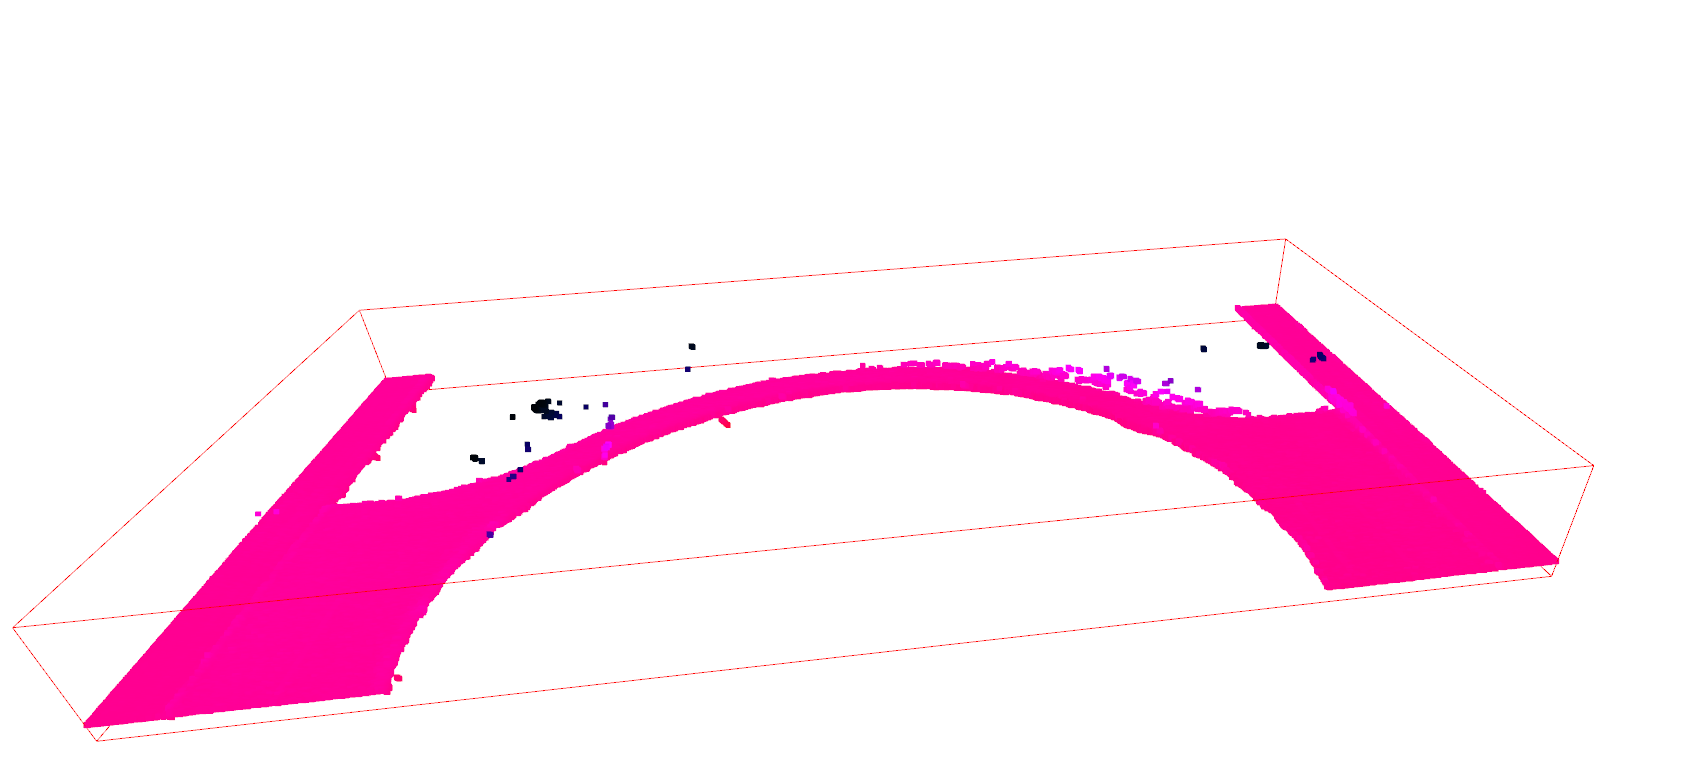
\includegraphics[width=0.4\textwidth]{images/pointcloud_big.PNG}
        \smallskip\par
        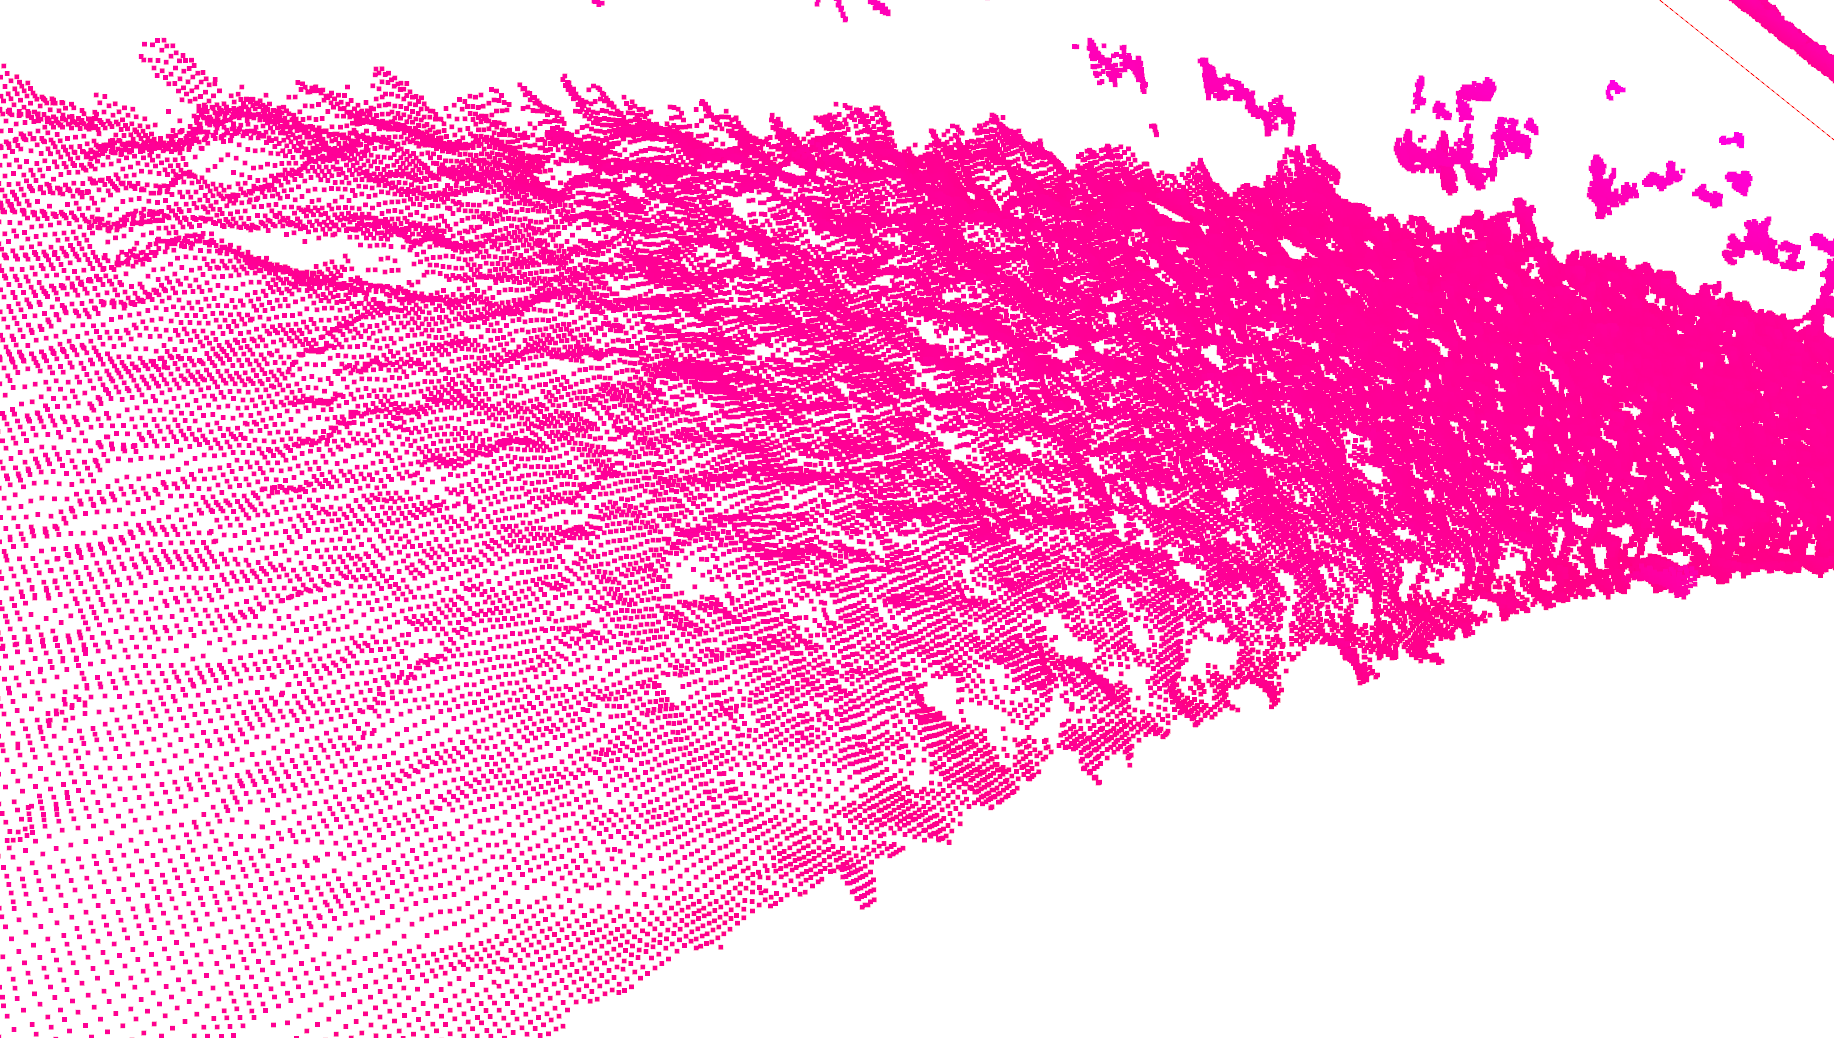
\includegraphics[width=0.4\textwidth]{images/pointcloud_small.PNG}
    \end{center}
    \caption{Pointcloud Komplett}
    \label{fig:pointclouds}
\end{wrapfigure}



Bevor ich mich aber mit dem 2. Schritt des Verfahrens beschäftige möchte ich auf die 
Datenstruktur von Pointclouds eingehen. Wie der Name schon sagt bestehende
Pointclouds aus Punkten. In unserem Fall ca. 3 Millionen für eine einzelene
Bewegung in X-Richtung. In jedem Punkt sind mindestens 3 Koordinaten gespeichert, 
Eine X und Y Koordinate relativ zu Ursprung der Pointcloud und eine Z Koordinate 
in der die Höhe gespeichert wird. Der Ursprung der Pointcloud liegt in der Mitte 
der X-Achse, also genau da wo der Scanner verläuft.
Zusätzlich ist für jeden Punkt auch noch eine Farbe als RGB-Farbwert
(3 Werte von 0 bis 255) gespeichert. Die Farbe wird relativ zu der Höhe
berechnet. Punkte bekommen einen Farbwert zugewiesen je nachdem wie nah 
sie an dem Minimum oder Maximum der Z-Koordinate sind. 
In \ref{fig:pointclouds} ist die komplette Pointcloud eines Demonstratorbauteils 
zu sehen, zusammen mit einer BoundingBox, durch diese werden die Randpunkte
der Pointcloud visuell dargestellt. Man sieht außerdem das unten liegende Punkte
hell und weiter oben liegende Punkte dunkler dargestellt werden.
Unterhalb ist eine Nahaufnahme des Mittelstücks des gleichen Bauteils zu sehen. 
Hier sind die einzelenen Punkte sichtbar.

Die Koordinaten sind als Float gespeichert haben keinerlei bezug zueiander.
Das heißt die X und Y Koordinaten sind nicht zum Beispiel anhand eines Grids 
angelegt, sondern können einen beliebigen Abstand zwischeneinander haben. Das
werden wir auch später in der weiteren Bearbeitung der Pointclouds sehen.

Wenn nun also alle Pointclouds für ein Objekt erfasst wurden kann zu dem 2.
Schritt des Verfahres übergegangen werden. Hier müssen die Daten zusammengefügt 
werden. 
Hierfür existieren in der Literatur schon verschiedene Verfahren, ein 
besonders beliebtes ist der ICP-Algorithmus.
Dieser Algorithmus existiert schon seit dem Beginn der 90ziger Jahre und ist 
der klassische Methode wenn es um die Registrierung von Pointclouds und 
anderen Punkt-Sets geht. \cite[]{icp}
Der Algorithmus errechnet eine lokale, optimale Transformation die ein Datenset
dem anderen annähren kann. \cite{icp_og}
Um diese Transformation zu bestimmen werden zuerst die Distanzen von allen 
Punkten in Datenset A zu dem jeweils nähsten Punkt in Datenset B aufsummiert 
werden. Dann wird eins der Datensets verschoben und rotiert und wieder die 
Distanzen gebildet. Dies wird solange gemacht bis die Änderung der Distanzen 
konvergiert. Die enstehende Transformation ist dann optimal.
Für identische Datensets die sich nur in einer Transformation und Rotation 
unterscheiden, funktioniert dieser Algorithmus sehr gut. Bei Datensätzen die 
Messfehler oder Überlappungen beeinhalten kann häufig keine Optimale 
Transformation bestimmt werden.
Deswegen wurden seit der ersten Vorstellung des Algorithmus viele Varianzen
entwickelt die mit diesem Schwächen umgehen. 
Zum Beispiel der 'Sparse Iterative Closest Point' Algorithmus von \cite{Bouaziz.2013}
oder die 'Anderson-accelerated' Version die besser mit Außreißern und nur 
partiell überlappenden Daten umgehen kann und eine gleichwertige oder bessere 
Transformation errechnen kann. \cite{icp}

Aufgrund der Versprechen dieses Varianten und weil dieser Algorithmus in vielen
Open-Source Bibliotheken schon implementiert ist war das auch mein erster Ansatz
und ich habe mit Hoffnungen gemacht das, das zusammenzufügen der Pointclouds 
damit schnell abgehakt ist.




\end{document}